\documentclass{book}
\usepackage{graphicx}
\usepackage[english]{babel}
\usepackage{amsthm}
\usepackage{amssymb}
\usepackage{amsfonts}
\usepackage{mdframed}
\usepackage{physics}
\usepackage{tikz}
\usepackage[a4paper, margin=1in]{geometry}
\geometry{a4paper, margin=1in}
\usepackage{xcolor}
\usetikzlibrary{arrows.meta}
\usetikzlibrary{angles,quotes}
\graphicspath{ {./images/} }
\usepackage{svg}
\usepackage{subcaption}
\usepackage{bm}
\usepackage{empheq}
\usepackage{cancel}
\usetikzlibrary{decorations.text}
\usepackage[most]{tcolorbox}
\usepackage{tensor}
\usetikzlibrary{patterns.meta}
%3D
\usepackage{mathtools}
\usepackage{booktabs}
\usepackage{array}
\newcolumntype{C}{>{$}c<{$}}
\usepackage{tikz-3dplot}
\usepackage{appendix}
\usepackage{pgfplots}
\usetikzlibrary{shapes.geometric}
\usetikzlibrary{calc,patterns,angles,quotes}
%Tikz Library
\usetikzlibrary{angles, quotes, intersections}
\usepackage[bb=dsserif]{mathalpha}
\usetikzlibrary{decorations.pathmorphing}

\tikzset{snake it/.style={decorate, decoration=snake}}

\usepackage{etoolbox} % ifthen
\usepackage[outline]{contour} % glow around text
\usetikzlibrary{calc} % for adding up coordinates
\usetikzlibrary{decorations.markings,decorations.pathmorphing}
\usetikzlibrary{angles,quotes} % for pic (angle labels)
\usetikzlibrary{arrows.meta} % for arrow size
\usepackage{xfp} % higher precision (16 digits?)

\usepackage{tcolorbox}

%https://osl.ugr.es/CTAN/macros/latex/contrib/tcolorbox/tcolorbox.pdf
\tcbuselibrary{breakable}
\tcbset{%any default parameters
	width=0.7\textwidth,
	halign=justify,
	center,
	breakable,
	colback=white    
}

\newenvironment{aside}
{\begin{mdframed}[style=0,%
		leftline=false,rightline=false,leftmargin=2em,rightmargin=2em,%
		innerleftmargin=0pt,innerrightmargin=0pt,linewidth=0.75pt,%
		skipabove=7pt,skipbelow=7pt]\small}
	{\end{mdframed}}

\renewcommand{\cleardoublepage}{\clearpage}
\newcommand{\dbar}{\mathrm{d}\hspace*{-0.08em}\bar{}\hspace*{0.1em}}
\title{Statistical Mechanics}
\author{Dominik Szablonski}
\newtheorem{law}{Law}
\newtheorem{klaw}{Law}

\newtcbtheorem{Definitions}{Definition}%
{colback=blue!5!white,colframe=blue!75!black,width=\textwidth,fonttitle=\bfseries}{}

\newtcbtheorem{Theorems}{Theorem}%
{colback=red!5!white,colframe=red!75!black,width=\textwidth,fonttitle=\bfseries}{}

\newtcbtheorem{Postulates}{Postulate}%
{colback=green!5!white,colframe=green!75!black,width=\textwidth,fonttitle=\bfseries}{}

\newtheorem*{theorem}{Theorem}


\setlength\parindent{0pt}
\pgfplotsset{compat=1.18}
\begin{document}
\maketitle

\tableofcontents

\chapter{Basic Thermodynamics}
We will begin by discussing systems with variable particle number. In order to talk as system where the number of particles $N$ varies, we must consider its \textit{chemical potential}, which is defined in terms of the Gibbs free energy,
\begin{equation}
	\mu = \eval{\pdv{G}{N}}_{T,P}.
\end{equation} 
We can find a simpler expression for the chemical potential by considering,
\begin{equation}
	G = G(N,\underbrace{P,T}_{\text{intensive}}).
\end{equation}
We know that the Gibbs free energy is an extensive variable, and so is the number of particles $N$. Thus, we can write,
\begin{equation}
	G = Nf(P,T)
\end{equation}
where $f$ is some function. We actually ind that $f(P,T) = \mu$, so we can write,
\begin{equation}
	\mu = \frac{G}{N}
\end{equation}
from which we can also conclude that $\mu$ is a function of $P$ and $T$. Let us now attempt to generalise this to more than one species of gas. This means that there is more than one extensive variable. For now, let us state without proof,
\begin{equation}
	G = \sum_i \mu_i N_i
\end{equation}
where $N_i$ is the number of particles of a particularly species and $\mu_i$ is its chemical potential. We can then write,
\begin{equation}
	\mu_i = \mu_i\left(T, P, \left\{\frac{N_j}{N}, \forall j \in \mathbb{N}\right\}\right).
\end{equation}
However, if we consider an ideal gas, we can ignore interactions due to other species of gas so we can simply consider, $\mu_i = \mu_i(T, P, N_i/N)$. However,
\begin{align}
	P & = \frac{1}{V}Nk_BT  = \sum_i P_i  & N = \sum_i N_i \\
	& &P_i = \frac{N_i}{V}k_BT \to \text{ Partial pressure} \\
	\implies && \mu_i = \mu_i (T, P_i).
\end{align}
Let us return to considering a single species, and recall,
\begin{align}
	\dd{S} = \frac{1}{T}\dd{E} + \frac{P}{T}\dd{V} && \dd{E} = C_V\dd{T} && V = \frac{Nk_BT}{P}
\end{align}
from which we can show,
\begin{equation}
	- \Delta S = C_P\ln\frac{T}{T_0} - Nk_B\ln\frac{P}{P_0}
\end{equation}
\section{Constant Temperature}
At constant temperature, the Gibbs free energy is,
\begin{align}
	&\Delta G = - T \Delta S = Nk_BT\ln\frac{P}{P_0} \\
	\implies & \Delta \mu = k_BT_0 \ln\frac{P}{P_0}.
\end{align}
\subsection{Chemical Reactions}
If we consider two gasses separated by a membrane, the chemical potential will govern the diffusion of the gasses, and the partial pressures will tend to equalise. Let us consider a reaction between two substances, $A \rightleftharpoons B$. The Gibbs free energy is,
\begin{equation}
	\dd{G} = \mu_A\dd{N}_A + \mu_B \dd{N_B}
\end{equation}
however $\dd{N}_B = \dd{N}_A$, so,
\begin{equation}
	\dd{G} = (\mu_A - \mu_B)\dd{N}_A.
\end{equation}
We have equilibrium when a small change in $N_A$ leaves $G$ unchanged, so $\mu_A = \mu_B$.
\\\\
Let us now consider a reaction with double the reactants and products, $aA + bB \rightleftharpoons xX + yY$, where $a,b,x,y \in \mathbb{Z}$. The number of molecules change by,
\begin{align}
	\dd{N}_B = \frac{b}{a}\dd{N}_A && \dd{N}_X = -\frac{x}{a}\dd{N}_A
\end{align}
Let us write the Gibbs free energy,
\begin{equation}
	\begin{split}
		\dd{G} & = \mu_A\dd{N}_A + \mu_B\dd{N}_B - \mu_X\dd{N}_X - \mu_Y\dd{N}_Y \\ 
		& = \underbrace{\left(\mu_A + \frac{b}{a}\mu_B - \frac{x}{a}\mu_X - \frac{y}{a}\mu_Y\right)}_{0\text{ at equilibrium}}\dd{N}_A \\
		\implies & \mu_A+ b\mu_B = x\mu_X + y\mu_Y
	\end{split}
\end{equation}
We wish to work in terms of moles, so let us write the molar Gibbs free energy,
\begin{equation}
	g^r = xg_X + yg_Y - ag_A - bg_B
\end{equation}
which will be 0 at equilibrium. If we know the $g^r_0 \equiv g_r(T_0, P_0)$ at some reference temperature and partial pressure for all reactants and products, then we can find the molar Gibbs free energy at other partial pressures but the same temperature. Applying our ideal gas assumptions,
\begin{equation}
	\begin{split}
		g_r\left(\left\{P_i\right\},T_0\right) & = g_r(P_0,T_0) + N_Ak_BT_0\left(x\ln\frac{P_X}{P_0} + y\ln\frac{P_Y}{P_0} - a\ln\frac{P_A}{P_0} - b\ln\frac{P_B}{P_0}\right) \\ 
		& = g_r(P_0, T_0) + \ln\left(\left(\frac{P_X}{P_0}\right)^x\left(\frac{P_Y}{P_0}\right)^y\left(\frac{P_0}{P_A}\right)^a\left(\frac{P_0}{P_B}\right)^b\right).
	\end{split}
\end{equation}
At equilibrium $g_r$ = 0, so,
\begin{equation}
	\underbrace{\left(\frac{P_X}{P_0}\right)^x\left(\frac{P_Y}{P_0}\right)^y\left(\frac{P_0}{P_A}\right)^a\left(\frac{P_0}{P_B}\right)^b}_{Q} = \underbrace{\exp\left(-\frac{g_0^r}{RT_0}\right)}_{K_P(T_0)}.
\end{equation}
%and we find,
%\begin{align}
%	Q > K_P && A,B \to X,Y \\
%	Q < K_P && X,Y \to A,B \\
%	Q = 0 && \text{Equilibrium}.
%\end{align}
We can write more generally, an equation for $N$ reactants and $N'$ products,
\begin{equation}
	g_r = \sum_{i=1}^{N'}x_ig_{X_i} - \sum_{j=1}^Na_jg_{A_j}
\end{equation}
and at equilibrium,
\begin{equation}
	\prod_{i=1}^{N'}\left(\frac{P_{X_i}}{P_0}\right)^{x_i}\sum_{j=1}^{N}\left(\frac{P_0}{P_{A_j}}\right) = \exp\left(-\frac{g_0^r}{RT_0}\right)
\end{equation}
\chapter{Statistical Physics}
Before jumping into statistical physics, we must define a few terms,
\begin{Definitions}{Macrostate}{}
	State of a sufficiently large system in equilibrium specified by a few measurable quantities, i.e., $P$, $T$, etc.
\end{Definitions}
\begin{Definitions}{Microstate}{}
	A description of a system consisting of the position and momentum (or quantum states) of every molecule present in the system.
\end{Definitions}
We wish to relate the macrostate to the microstate and predict macroscopic properties from first principles. For each macrostate, there exist many microstates. In order to formulate statistical mechanics, we must assume that a system can access al available microstates, so we can average over al microstates to predict the macrostate.
\section{Microcanonical Ensemble}
\begin{Definitions}{Ensemble}{}
	Collection of objects, which are copies of the system at each point in time. 
\end{Definitions}
We use the ensemble to avoid taking time averages. The ensemble average is given by,
\begin{equation}
	\left<x\right> = \sum_i P_iX_i
\end{equation}
where $P_i$ is the probability of the $i$th microstate, and $X_i$ is the value of $X$ in the $i$th microstate. Let us now say that we have $\nu$ objects in the ensemble, with $\nu_i$ objects in the $i$th microstate, and we denote each object in the ensemble with $\lambda$, we can write,
\begin{equation}
	\left<x\right>  = \frac{1}{\nu} \sum_{\lambda}X_{\lambda} = \frac{1}{\nu}\sum_i\nu_iX_i = \sum_i P_iX_i
\end{equation}
from which we find,
\begin{equation}
	P_i = \frac{\nu_i}{\nu}.
\end{equation}
However, for a system in isolation, we can postulate the following,
\begin{Postulates}{Postulate of Equal a priori Probabilities}{}
	All microstates are equally likely.
\end{Postulates}
Thus, if our total number of microstates is $\Omega$, the probability of the $i$th microstate is,
\begin{equation}
	P_i = \frac{1}{\Omega},\hspace{1em}\forall i.
\end{equation}
\begin{aside}
	For a system with $N$ particles which each can be in one of two states, such that there are $n$ and $N-n$ states respectively, then the total number of microstates is given by,
	\begin{equation}
		\frac{N!}{n!(N-n)!} = {^nC_N}.
	\end{equation}
\end{aside}
\section{Statistical Basis of Entropy}
The number of microstates $\Omega$ for a number of particles $N$ in the system and a set of particles of size $n$ in one state, $m$ in a second state, etc., is given by,
\begin{equation}
	\Omega(n) = \frac{N!}{n!m!\cdots!}.
\end{equation}
For a system with just $N$ total particles and two sets of particles of size $n$, $N-n$ this is,
\begin{equation}
	\Omega(n) = \frac{N!}{n!(N-n)!}.
\end{equation}
For large systems, $\Omega$ rises dramatically. For two possible states, we can write the distribution of microstates as a binomial distribution,
\begin{align}
	\overline{n} = \frac{N}{2} && \sigma_n = \frac{\sqrt{N}}{2} && \frac{\sigma_n}{N} \approx \frac{1}{\sqrt{N}}.
\end{align}
For large $N$, we find that the ensemble average $\left<X\right>$ is entirely dominated by microstates with the most probable $X_i$, denoted $X_{\text{Prob}}$. Thus,
\begin{equation}
	\langle X \rangle = \sum_i P_i X_i \approxeq X_{\text{Prob}}
\end{equation}
which is true within a few $\sigma$ of the most probable value.
\\\\
As the microstate changes, the vast majority of new states have similar (or essential equal) $X_i \approx X_{\text{Prob}}$ so nothing changes at equilibrium.
\\\\
If our system begins out of equilibrium, i.e., $n < N/2$, the time evolution must in principle increase or decrease $n$, but there are vastly more states with greater $n$ and so evolution is overwhelmingly likely to lead to $n \uparrow$ until $n \approx N/2$. 
\\\\
Furthermore, for large $N$, $\Omega(n)$ tends to an exponential,
\begin{equation}
	\Omega(n) = \exp\left(\frac{\left(n - \frac{N}{2}\right)^2}{\frac{N}{2}}\right)
\end{equation}
with mean $N/2$, $\sigma = \sqrt{N}/2$.
\\\\
We might then think that $\Omega \propto S$, but this is not the case. This is because entropy is extensive, whereas we combine microstates by multiplying them together. Instead, the following relation holds,
\begin{equation}
	S = k_B \ln\Omega.
\end{equation}
\section{Spin-Half Paramagnet}
An atom or molecule of a spin-$\frac{1}{2}$ paramagnet has $s = \frac{1}{2}$, $\abs{\vb{S}} = \frac{\sqrt{3}}{2}\hbar$, $S_z = \pm \frac{1}{2}\hbar$. Each molecule has a magnetic moment $\vb*{\mu}$ such that $\mu_z = \pm \mu$. The total magnetisation of the sample is then given by,
\begin{equation}
	\begin{split}
		m & = n_{\uparrow} + n_{\downarrow}(-\mu) \hspace{2em} n_{\downarrow} = N - n_{\uparrow} \\
		& = (2n_{\uparrow} - N)\mu	\end{split}
\end{equation}
If there is a magnetic field, the energy is given by,
\begin{equation}
	 U = -\vb{m}\cdot\vb{B}
\end{equation}
with each atom having energy $\mp \mu B$ for spin $\updownarrow$, as the atoms align to lower energy. The total energy is then,
\begin{equation}
	U = n_{\uparrow}(-\mu B) + n_{\downarrow}(\mu B) = (N - 2n_{\uparrow})\mu B = mB.
\end{equation}
The microstates are then specified by specifying the spin of each atom. For $N$ atoms there are $2^N$ microstates. If there is no external magnetic field, the atoms have equal probability of being $\uparrow$ or $\downarrow$, thus equilibrium will be reached at $m=0$.
\subsection{Energy to Temperature}
\begin{figure}
	\centering
	\begin{tikzpicture}
		\draw (0,0) rectangle (4,4);
		\fill[pattern={Lines[angle=45,distance=0.5cm]}] (0,4) rectangle (4,4.25);
		\fill[pattern={Lines[angle=45,distance=0.5cm]}] (0,0) rectangle (-0.25,4);
		\fill[pattern={Lines[angle=45,distance=0.5cm]}] (0,0) rectangle (4,-0.25);
		\fill[pattern={Lines[angle=45,distance=0.5cm]}] (4,4) rectangle (4.25,0);
		\draw[dashed] (2,0.1) -- (2,3.9);
		\draw (1.9,0.1) -- (2.1,0.1);
		\draw (1.9,3.9) -- (2.1,3.9);
		\node at (1,3) {$E_1$};
		\node at (1,2) {$N_1$};
		\node at (1,1) {$V_1$};
		\node at (3,3) {$E_2$};
		\node at (3,2) {$N_2$};
		\node at (3,1) {$V_2$};
	\end{tikzpicture}
	\caption{}
	\label{fig:isolated}
\end{figure}
Let us consider an isolated system separated by a permeable membrane, as in figure \ref{fig:isolated}, such that,
\begin{align}
	E_1 + E_2 = E && N_1 + N_2 = N && V_1 + V_2 = V
\end{align}
are fixed. We further have,
\begin{align}
	\Omega = \Omega_1 + \Omega_2 && S = k_B\ln\Omega_1 + k_B\ln\Omega_2 = S_1 + S_2.
\end{align}
Let us consider the heat flow in the system only, keeping $V_1,V_2$ and $N_1,N_2$ constant. We have,
\begin{equation}
	\dd{S} = \left(\pdv{S_1}{E_1}\right)_{V_1,N_1}\dd{E_1} + \left(\pdv{S_2}{E_2}\right)_{V_2,N_2}\dd{E_2}
\end{equation}
however, $\dd{E}_1 = - \dd{E}_2$, so,
\begin{equation}
	\dd{S} = \left(\left(\pdv{S_1}{E_1}\right)_{V_1,N_1} - \left(\pdv{S_2}{E_2}\right)\right)\dd{E}_1
\end{equation}
and equilibrium is reached when,
\begin{equation}
	\left(\pdv{S_1}{E_1}\right)_{V_1,N_1} = \left(\pdv{S_2}{E_2}\right)_{V_2,N_2}
\end{equation}
this equation thus governs heat transfer. If $\dd{E} > 0$, then $\dd{S} >0$ and,
\begin{equation}
	\left(\pdv{S_1}{E_1}\right)_{V_1,N_1} > \left(\pdv{S_2}{E_2}\right)_{V_2,N_2}
\end{equation}
so heat flows from high $\left(\pdv{S}{E}\right)_{V,N}$  to low $\left(\pdv{S}{E}\right)_{V,N}$, so we require $T$ to decrease with $\left(\pdv{S}{E}\right)_{V,N}$. Furthermore, $\left(\pdv{S}{E}\right)_{V,N} > 0$ for almost al systems, so an appropriate guess would be to say,
\begin{equation}
	\left(\pdv{S}{E}\right)_{V,N} = \frac{1}{T}. \label{eq:1/T}
\end{equation}
Repeating similar process, but only allowing $V_1, V_2$ to vary, we find that $\left(\pdv{S}{V}\right)_{E,N}$ governs how the partition moves. If $\left(\pdv{S_1}{V_1}\right)_{E_1,N_1} > \left(\pdv{S_2}{V_2}\right)_{E_2,N_2}$, we have that $V_1$ increases and $V_2$ decreases, like pressure. Thus, we can link this to classical thermodynamics,
\begin{equation}
	\left(\pdv{S}{V}\right)_{E,N} = \frac{P}{T}.
\end{equation}
Considering variable particle number, we obtain,
\begin{equation}
	\left(\pdv{S}{N}\right)_{V,E} = \frac{\mu}{T}
\end{equation}
and thus, we can obtain the fundamental thermodynamic relation,
\begin{equation}
	\dd{S} = \frac{1}{T}\dd{E} + \frac{P}{T}\dd{V} - \frac{\mu}{T}\dd{N}.
	\end{equation}
\subsection{Isolated spin-$\frac{1}{2}$ paramagnet in the presence of a magnetic field}
Let us return to the ideal paramagnet. The total energy is given by,
\begin{equation}
	E = \mu B \left(N - 2n_{\uparrow}\right) = \mu B \left(2n_{\downarrow} - N\right).
\end{equation}
The reversible work done is,
\begin{equation}
	\dbar W^{\text{rev}} = -m\dd{B} \implies \frac{m}{T} = \left(\pdv{S}{B}\right)_{E,N}.
\end{equation}
The entropy of the paramagnet is,
\begin{equation}
	\begin{split}
	S & = k_B \ln \Omega(E, B) \\
	& = k_B ln\left(\frac{N!}{n_{\uparrow}!\left(N - n_{\uparrow}\right)!}\right).
	\end{split}
\end{equation}
where $\Omega$ is a function of $E,B$ as $n_{\uparrow}$ and $E$ co-vary as,
\begin{equation}
	n_{\uparrow} = \frac{1}{2}\left(N - \frac{E}{\mu B}\right).
\end{equation}
We will use Stirling approximation,
\begin{equation}
	\ln (x!) = x\ln x - x \label{eq:stiring}
\end{equation}
which holds for large $x$. By writing out,
\begin{equation}
	S = k_B \left[\ln(N!) - \ln(n_{\uparrow}!) - \ln \left((N-n_{\uparrow})!\right)\right]
\end{equation}
and using equation \eqref{eq:stiring},
\begin{equation}
	S = k_B\left[N\ln(N) - n_{\uparrow}\ln(n_{\uparrow}) - (N-n)\ln(N-n)\right]
\end{equation}
While in equilibrium, $n_{\uparrow} = n_{\downarrow} = \frac{N}{2}$, in which case,
\begin{equation}
	S = k_B\ln(2^N)
\end{equation}
which indicates that essentially all microstates are at equilibrium. Applying the chain rule to equation \eqref{eq:1/T}, we find,
\begin{equation}
	\frac{1}{T} = \left(\pdv{S}{n_{\uparrow}}\right)_{N}\left(\pdv{n_{\uparrow}}{E}\right)_B.
\end{equation}
We then find,
\begin{equation}
	\left(\pdv{S}{n_{\uparrow}}\right)_B = k_B \ln \frac{N - n_{\uparrow}}{n_{\uparrow}}
\end{equation}
and,
\begin{equation}
	\left(\pdv{n_{\uparrow}}{E}\right)_B = -\frac{1}{2\mu B}
\end{equation}
thus,
\begin{equation}
	\frac{1}{T} = \frac{k_B}{2\mu B}\ln \left(\frac{n_{\downarrow}}{n_{\uparrow}}\right).
\end{equation}
For the magnetic field,
\begin{equation}
	\frac{m}{T} = \left(\pdv{S}{B}\right)_{E,N} = \frac{k_BE}{2\mu B^2}\ln \left(\frac{n_{\downarrow}}{n_{\uparrow}}\right) \implies m = -\frac{E}{B}.
\end{equation}
For a varied magnetic field, we can write the ratio of spin-down to spin up electrons as,
\begin{equation}
	\frac{n_{\downarrow}}{n_{\uparrow}} = \exp\left(-\dfrac{2\mu B}{k_B T}\right). \label{eq:ratio}
\end{equation}
\section{The Ideal Gas}
We can derive the equation for a classical, ideal gas. Let us consider a volume divided into small cells, such that we can treat position microstates as discrete, of volume $\Delta V$. There are $V/\Delta V$ cells, and $\left(V/\Delta V\right)^N$ microstates. Thus, the entropy is,
\begin{equation}
	S = N k_B \ln\frac{V}{\Delta V}.
\end{equation}
We then find,
\begin{equation}
	\begin{split}
		\frac{P}{T} & = \left(\pdv{S}{V}\right)_{E,N} = Nk_B\frac{1}{V} \\
		& \implies PV = Nk_BT.
	\end{split}
\end{equation}
\chapter{Statistical Physics of Non-Isolated Systems}
In order to find the physics of non-isolated systems, we must fix $T$ and $E$. $\langle E \rangle$ depends on $T$, although there will be microscopic fluctuations. These fluctuations are of an order,
\begin{equation}
	\frac{\Delta E}{\langle E \rangle} \sim \frac{1}{\sqrt{N}}.
\end{equation}
\section{Boltzmann Distribution}
	\begin{figure}
		\centering
		\begin{tikzpicture}
			\draw (0,0) rectangle (4,4);
			\fill[pattern={Lines[angle=45,distance=0.5cm]}] (0,4) rectangle (4,4.25);
			\fill[pattern={Lines[angle=45,distance=0.5cm]}] (0,0) rectangle (-0.25,4);
			\fill[pattern={Lines[angle=45,distance=0.5cm]}] (0,0) rectangle (4,-0.25);
			\fill[pattern={Lines[angle=45,distance=0.5cm]}] (4,4) rectangle (4.25,0);
			\draw (3,0) -- (3,1) -- (4,1);
			\node at (1.5, 2.5) {$R$};
			\node at (1.5, 2) {$E_R$};
			\node at (3.5, 0.75) {$S$};
			\node at (3.5, 0.25) {$\varepsilon$};
		\end{tikzpicture}
		\caption{Isolated system consisting of large reservoir $R$ and small system $S$ such that $S << R$.}
		\label{fig:isolated2}
	\end{figure}
Consider an isolated system as in figure \ref{fig:isolated2}. The total energy of this system is fixed, such that $E = E_R + \varepsilon$. We wish to know, for the $i$th microstate of $S$, what is the probability $p_i$ of finding it in that microstate, with an associated energy $\varepsilon_i$. This probability is directly proportional to the total number of microstates,
\begin{equation}
	\begin{split}
		p_i & \propto \Omega_{S+R} = \Omega_S\Omega_R \\
		& \propto \Omega_R(E - \varepsilon_i) = e^{\frac{1}{k_BT}S_R(E - \varepsilon_i)}.
	\end{split}
\end{equation}
Given $E << \varepsilon_i$, we can perform a taylor expansion up to the first order,
\begin{equation}
	S_R(E - \varepsilon_i) = S_R(E) - \varepsilon_i\underbrace{\eval{\pdv{S_R}{E}}_{E_R = E}}_{\frac{1}{T}}.
\end{equation}
Thus, we have,
\begin{equation}
	p_i \propto e^{\frac{1}{k_B}S_R(E)}e^{-\frac{\varepsilon_i}{k_BT}}
\end{equation}
which we can write as,
\begin{align}
	p_i= \frac{1}{Z}e^{-\frac{\varepsilon_i}{k_BT}} && Z = \sum_je^{-\frac{\varepsilon_j}{k_BT}} \label{eq:Z}
\end{align}
which is the Boltzmann distribution, with normalisation $Z$.
\subsection{Paramagnet}
Let us consider a paramagnet consisting of a single atom. There are 2 states, $\uparrow E = -\mu B$ and $\downarrow E = \mu B$. Therefore, the normalisation is,
\begin{equation}
	Z = e^{\frac{\mu B}{k_BT}} + e^{-\frac{\mu_B}{k_BT}}
\end{equation}
and the probability of spin up and spin down are,
\begin{align}
	P(\uparrow) = \frac{e^{\frac{\mu B}{k_B T}}}{Z} && P(\uparrow) = \frac{-e^{\frac{\mu B}{k_B T}}}{Z}
\end{align}
whose ratio is,
\begin{equation}
	\frac{P(\downarrow)}{P(\uparrow)} = e^{-\frac{2\mu B}{k_BT}}
\end{equation}
which is identical to eq. \eqref{eq:ratio}.
\section{Partition Function}
The normalisation factor $Z$ in equation eq. \eqref{eq:Z} is also known as the \textit{partition function}. It is useful to us, as we are able to extract useful information about different macroscopic properties of a system. If we define $\beta = 1/k_BT$, we have,
\begin{align}
	\langle E \rangle & = \frac{\sum_i\varepsilon_ie^{\varepsilon_i\beta}}{\sum_j e^{-\varepsilon_j \beta}} = -\pdv{\ln(Z)}{\beta} \\
	\langle C_V \rangle & = \pdv{\langle E \rangle}{T} = -\frac{1}{k_BT^2}\pdv[2]{\ln(Z)}{\beta} \\
	\langle E^2 \rangle & = \frac{1}{Z}\pdv[2]{Z}{\beta}\\
	\Delta E^2 & = \left(k_B T\right)^2 \frac{C_V}{k_B}.
\end{align}
\section{Helmholtz Free Energy and Entropy}
We wish to consider a system larger than $S$. Let us consider $\nu$ copies of the system, all in thermal contact. This can be considered a canonical ensemble because, together, they are large enough to have a well defined $T$. Then, for any individual $S$, the rest of the system is the reservoir, whose probabilities follow the Boltzmann distribution.
\\\\
The ensemble has $\nu_i$ copies in the $i$th microstate, with $p_i = \nu_i/\nu$. The total number of microstates is,
\begin{equation}
	\Omega_{\nu} = \frac{\nu!}{\nu_1!\nu_2!\nu_3!\ldots},
\end{equation} 
and by Stirling's approximation,
\begin{equation}
	\begin{split}
	\ln\Omega_{\nu} &= \nu\ln\nu - \nu -\biggl(\sum_i \nu_i\ln\nu_i - \underbrace{\sum_j\nu_j}_{\nu}\biggr) \\
	& = \nu\ln\nu - \sum_i\nu_i\ln\nu_i \\ & = \sum_i\nu_i(\ln\nu - \ln\nu_i) \\
	& = \sum_i \nu_i\ln\frac{\nu}{\nu_i} \\
	& = -\sum_i\nu_i\ln p_i \\
	& = -\nu\sum_i p_i\ln p_i
	\end{split}
\end{equation}
and by extensivity,
\begin{equation}
	\begin{split}
		\langle S \rangle &= \frac{1}{\nu}\langle S_{\nu}\rangle \\
		& \boxed {= - k_B\sum_ip_i\ln p_i}
	\end{split}
\end{equation}
which is known as the \textit{Gibbs entropy}. Let us check if this works for the macrocanonical ensemble, i.e., $p_i = \frac{1}{\Omega}$. We have,
\begin{equation}
	\begin{split}
	\langle S \rangle &= k_B\sum_i^{\Omega}\frac{1}{\Omega}\ln \Omega \\
	& = k_B \Omega
	\end{split}
\end{equation}
which is what we expect. Furthermore, the Gibbs expression is more general and can be applied to any probability distribution. Let us now apply this to the canonical ensemble, with $p_i = e^{-\varepsilon_i\beta}/Z$,
\begin{equation}
	\begin{split}
	\langle S \rangle &= -k_B\sum_ip_i\left[\ln\left(e^{-\varepsilon_i\beta}\right)-\ln Z\right]\\
	& = -k_B \sum_ip_i\left(\varepsilon_i\beta - \ln Z\right) \\
	& = k_B \left(\frac{1}{k_B T}\langle E \rangle + \ln Z \right) \\
	& = \frac{1}{T} \pdv{\ln Z}{\beta} + k_B\ln Z = \frac{\left<E\right>}{T} + k_B\ln Z
\end{split}
\end{equation}
so we can find $\langle S \rangle$ from $Z$. However, we can rewrite this as,
\begin{equation}
	k_BT \ln Z = \langle E \rangle - T \langle S \rangle = \langle F \rangle \label{eq:F}
\end{equation}
so we find that $Z$ directly gives us $F(T,V)$ or $F(T,B)$, or the Helmholtz free energy. The Helmholtz free energy is the natural potential for a system at fixed energy. Let us then recall the Maxwell relations,
\begin{align}
	S = -\left(\pdv{F}{T}\right)_{V (\text{or } B), N} && P = -\left(\pdv{F}{V}\right)_{T, N} && \mu = \left(\pdv{F}{N}\right)_{V, T} \label{eq:maxwell}
\end{align}
\subsection{The paramagnet at fixed temperature}
\begin{figure}
	\centering
	\begin{subfigure}{0.45\textwidth}
		\centering
		\begin{tikzpicture}[scale=0.8]
			\begin{axis}[
				xlabel=$\beta$, 
				ylabel =$\langle E \rangle$, 
				domain=0:10,
				ymax=0.1,
				axis y line = left,
				axis x line = middle,
				ticks = none]
				\addplot[blue, samples=100] {-tanh(0.5*x)};
			\end{axis}
			\node at (-0.8,0.1) {$-N\mu B$};
		\end{tikzpicture}
		\caption{$\langle E \rangle$ vs. $\beta$.}
	\end{subfigure}
	\begin{subfigure}{0.45\textwidth}
		\centering
		\begin{tikzpicture}[scale=0.8]
			\begin{axis}[
				xlabel=$T$, 
				ylabel =$\langle E \rangle$, 
				domain=0:10,
				axis y line = left,
				axis x line = middle,
				ymax=0.1,
				ticks = none]
				\addplot[blue, samples=100] {-tanh(1.5/x)};
			\end{axis}
			\node at (-0.8,0.1) {$-N\mu B$};
		\end{tikzpicture}
		\caption{$\langle E \rangle$ vs. $1/T$.}
	\end{subfigure}
	\caption{Function of average energy against $\beta$ and $1/T$.}
	\label{fig:B}
\end{figure}
We had first considered a paramagnet consisting of a single atom, with a single spin, whose partition function is,
\begin{equation}
	Z_1 = e^{\mu B \beta} + e^{-\mu B \beta} = 2\cosh(\mu B \beta)
\end{equation}
and average energy,
\begin{equation}
	\left<E_1\right> = -\mu B \frac{2\sinh(\mu B \beta)}{2\cosh(\mu B \beta)} = -\mu B \tanh(\mu B \beta).
\end{equation}
We can see how this energy varies in figure \ref{fig:B}. We can also look at the heat capacity of the paramagnet,
\begin{equation}
	C_V = \left(\pdv{E}{T}\right)_{N,B} = Nk_b(\mu B \beta)^2\sech[2](\mu B \beta)
\end{equation}
which we visualise in figure \ref{fig:cv}.
\begin{figure}
	\centering
	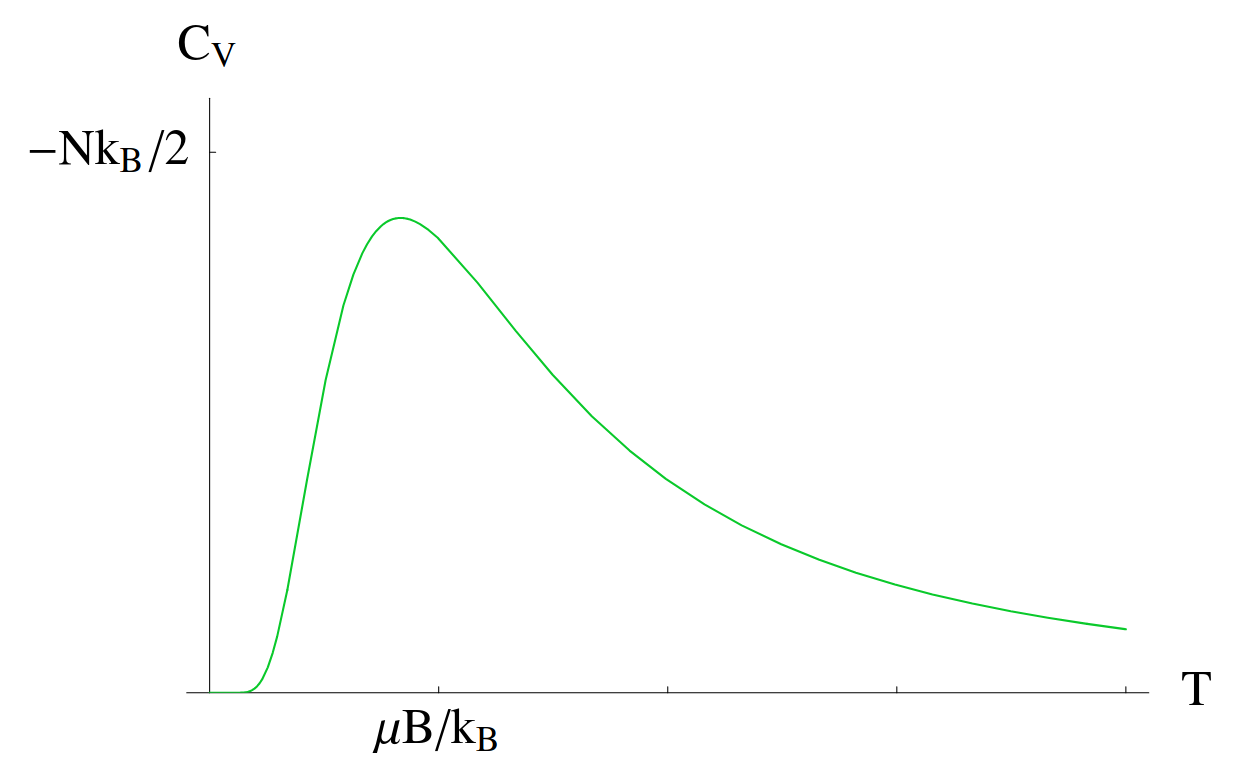
\includegraphics[width=0.45\textwidth]{cv.png}
	\caption{}
	\label{fig:cv}
\end{figure}
\\\\
For $N$ non-interacting spins, we can see that the energy will be $\langle E \rangle = N \langle \varepsilon_1 \rangle$. However, this does not hold for entropy. In order to progress to a paramagnet with $N$ spins, we require the partition function of the entire system, let us call this $Z_N$. This is given by,
\begin{equation}
	Z_N = (Z_1)^N.
\end{equation}
So,
\begin{equation}
	Z_N = \left(e^{\mu B \beta} + e^{-\mu B \beta}\right)^N
\end{equation}
and the Helmholtz free energy is,
\begin{equation}
	F = -Nk_BT\ln(Z_1)
\end{equation}
the entropy is,
\begin{equation}
	\langle S \rangle = N k_B \left(\ln(2\cos(\mu B \beta)) -\mu B \beta \tanh (\mu B \beta)\right)
\end{equation}
and the average magnetic dipole is,
\begin{equation}
	\left<m \right> = -\left<E\right>B.
\end{equation}
\section{Adiabatic Demagnetisation}
\begin{figure}
	\centering
	\begin{tikzpicture}
		\node at (-6,3) {$\downarrow$};
		\draw (0,0) -- (3,0) node[midway, anchor=north] {$10$};
		\draw (0,2) -- (3,2) node[midway, anchor = south] {$4$};
		\draw (-2,0.5) -- (-5,0.5) node[midway, anchor = north] {$10$};
		\draw (-2,1.5) -- (-5,1.5) node[midway, anchor = south] {$4$}; 
		\draw (5,0) -- (8,0) node[midway, anchor = north] {$8$};
		\draw (5,2) -- (8,2) node[midway, anchor = south] {$6$};
		\draw[-latex] (0,1) -- (-2,1) node[midway, anchor=north] {adiabatic};
		\node[anchor=south] at (-1,1) {work only};
		\draw[-latex] (3,1) -- (5,1) node[midway, anchor=south] {heat only};
		\node at (9,-1) {$\uparrow$};
	\end{tikzpicture}
	\caption{}
	\label{fig:magnetisation}
\end{figure}
\begin{figure}
	\centering
	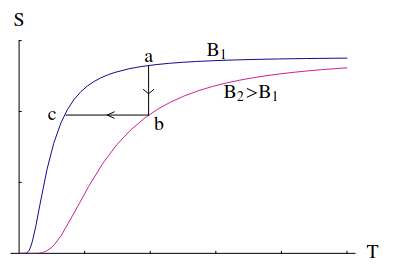
\includegraphics[width=0.3\textwidth]{magnet.png}
	\caption{}
	\label{fig:mag}
\end{figure}
Let us consider a system initially at a particular energy, we want to know its behaviour as we change temperature, energy, and/or heat. The energy is given by,
\begin{equation}
	\dd{E} = - m\dd{B} - B\dd{m}.
\end{equation}
where $m\dd{B}$ indicates work and $B\dd{m}$ indicates heat. Consider figure \ref{fig:magnetisation}. If we perform work on the magnet, we find that we do not change the spin ratio, so we decrease the magnetic field within the paramagnet, increase its energy, and decrease its temperature. This process is known as \textit{adiabatic demagnetisation}. If we look at figure \ref{fig:mag}, we find that we can change the temperature of a paramagnet by magnetising and demagnetising it. We lower the temperature in two steps,
\begin{enumerate}
	\item Have a sample in contact with a heat bath at $T_1$, and increase the magnetic field to $B_1$, known as \textit{isothermal magnetisation}.
	\item Reduce the field to $B_1$ slowly, to perform adiabatic demagnetisation. The temperature of the sample has now been decreased without changing the entropy or magnetisation.
\end{enumerate}
Let us note that we can perform this process for subsystems, however it will take infinite steps to reach 0K. There is always a minimum energy ground state $\varepsilon$, and for $k_BT << \varepsilon$, the probability of being in the ground state tends to 1 and the entropy tends to 0. 
\\\\
For $T \to \infty$, we find that $S \to \text{const}$, however this is only the case for systems with a finite number of microstates. In this case, the probability of each state is equal.
\section{Energies of Diatomic Molecules}
\subsection{Vibrational Energies}
The energy levels for a simple harmonic oscillator are,
\begin{equation}
	\varepsilon_n = \left(n + \frac{1}{2}\right)\hbar \omega, n \in \mathbb{Z}
\end{equation}
For a single oscillator, the partition function is,
\begin{equation}
	\begin{split}
		Z_1 & = e^{-\varepsilon_0\beta} + e^{-\varepsilon_1\beta} + e^{-\varepsilon_2 \beta} + \cdots  \\
		&  = e^{-\frac{1}{2}\hbar\omega\beta}\sum_{n=0}^{\infty}e^{-n\hbar\omega\beta}
	\end{split}
\end{equation}
which is a geometric series, so can be evaluated,
\begin{equation}
	Z_1 = \frac{e^{-\frac{1}{2}\hbar\omega\beta}}{1-e^{-\hbar\omega\beta}} = \frac{1}{2\sinh(\frac{\hbar\omega\beta}{2})}.
\end{equation}
From this we can evaluate the average energy,
\begin{equation}
	\begin{split}
	\left<E_1\right> &= \pdv{\beta}\left[\ln2 +\ln\left(\frac{\hbar\omega\beta}{2}\right) \right]\\
	& = \frac{\hbar\omega}{2}\frac{\cosh\left(\frac{\hbar\omega\beta}{2}\right)}{\sinh\left(\frac{\hbar\omega\beta}{2}\right)} = \frac{\hbar\omega}{2}\text{cotanh}\left(\frac{\hbar\omega\beta}{2}\right).
	\end{split}
\end{equation}
Analysing the limits as $T \to 0$, we find that $\text{cotanh}\left(\frac{\hbar\omega\beta}{2}\right) \to 1$, and $E \to \frac{\hbar \omega}{2}$, which is the ground state, and what we expect at low temperatures. In the limit $T \to \infty$, $\text{cotanh}\left(\frac{\hbar\omega\beta}{2}\right) \to \frac{1}{x}$, thus $E \to k_BT$, which is what we expect as this is a result of the equipartition theorem.
\section{Translational Energies of a Molecule in an Ideal Gas}
Consider a particle confined in a 3D box, i.e., in a potential,
\begin{equation}
	V(x,y,z) = \begin{cases}
		\infty &x > L_x \\
		\infty &y > L_y \\
		\infty &z > L_z \\
		0  & \text{Otherwise}
	\end{cases}
\end{equation}
for which the Schrodinger equation is,
\begin{equation}
	-\frac{\hbar^2}{2m}\laplacian{\psi} = E\psi
\end{equation}
with boundary conditions, $\psi(L_x,L_y,L_z) = \psi(0,0,0) = \psi(L_x,0,0) = \cdots = 0$. Thus, the solution will have a form,
\begin{equation}
	\psi = A\sin\left(\frac{n_x\pi}{L_x}x\right)\sin\left(\frac{n_y\pi}{L_y}y\right)\sin\left(\frac{n_z\pi}{L_z}z\right).
\end{equation}
And our energy levels are given by,
\begin{equation}
	E = \frac{\hbar^2 \pi^2}{2m}\underbrace{\left(\frac{n_x^2}{L_x} + \frac{n_x^2}{L_y^2} + \frac{n_z^2}{L_z^2}\right)}_{k^2}
\end{equation}
where $k = \abs{\vb{k}}$. The partition function is then given by,
\begin{equation}
	Z_1 = \sum_{n_x,n_y,n_z}^{\infty} e^{-E(n_x,n_y,n_z)\beta}
\end{equation}
which we can separate into 3 sums,
\begin{equation}
	\begin{split}
	Z_1 & = \left(\sum_{n_x=1}^{\infty} e^{-\frac{\hbar^2\pi^2}{2m}n_x^2\beta}\right)\left(\sum_{n_y=1}^{\infty} e^{-\frac{\hbar^2\pi^2}{2m}n_y^2\beta}\right)\left(\sum_{n_z=1}^{\infty} e^{-\frac{\hbar^2\pi^2}{2m}n_z^2\beta}\right)\\
	& = \left(\int_0^{\infty}e^{-\frac{\hbar^2}{2m}\beta k_x^2}\frac{L_x}{\pi}\dd{k_x}\right)\left(\int_0^{\infty}e^{-\frac{\hbar^2}{2m}\beta k_y^2}\frac{L_y}{\pi}\dd{k_y}\right)\left(\int_0^{\infty}e^{-\frac{\hbar^2}{2m}\beta k_z^2}\frac{L_z}{\pi}\dd{k_z}\right)
	\end{split}
\end{equation}
which are Gaussian integrals,
\begin{equation}
	\begin{split}
	Z_1 &= \frac{L_xL_yL_z}{2^3\pi^3}\left(\frac{2m\pi}{\hbar^2\beta}\right)^{\frac{3}{2}} \\
	& = V\underbrace{\left(\frac{mk_BT}{2\pi\hbar^3}\right)^{\frac{3}{2}}}_{g_sn_Q}
\end{split}
\end{equation}
where $n_Q = n_Q(T)$ known as the \textit{quantum concentration}, with dimensions of number density. We were able to convert the sums to integrals as even for every low temperatures, the energy spacing is much higher than the spacing between the energy levels, so we can use the continuum limit. We can then proceed to find the average energy,
\begin{equation}
	\left<E_1\right> = \frac{3}{2}k_BT
\end{equation}
as expected.
\subsection{The density of states}
Let us return to the particle in a box, and lets assume we cannot factorise the integral. We can then evaluate the integral over $k$-space in spherical polars,
\begin{equation}
	\begin{split}
	Z_1 &= \frac{V}{\pi^3}\int_0^{\infty}\int_0^{\frac{\pi}{2}}\dd{\theta}_k\int_0^{\frac{\pi}{2}}\dd{\phi}_kk^2e^{-\varepsilon(k)\beta}\sin\theta_k\dd{k} \\
	& = \frac{V}{\pi^3}4\pi\int_0^{\infty}k^2e^{-\frac{\hbar^2\beta}{2m}k^2}\dd{k} \\
	& = Vg_sn_Q
	\end{split}
\end{equation}
as before. $g_s = 2s+1$ is an additional degeneracy factor corresponding to the spin of the particles. Often $s=1/2$. It is useful to write this integral as,
\begin{equation}
	Z_1 = \int_0^{\infty}g(k) e^{-\varepsilon(k)\beta}\dd{k}
\end{equation}
where $g(k)$ is a degenerate factor, representing many states with the same energy, but different direction in $k$-space. We can find $g(k)$ by considering how many states lie in a thin strip $k \to k + \dd{k}$, i.e., the volume of a spherical shell in $k$ space and the volume per state,
\begin{equation}
	g(k) = \frac{1}{8}4\pi^2k^2\dd{k}\cdot \frac{1}{\frac{\pi}{L_x}\frac{\pi}{L_y}\frac{\pi}{L_z}} = \frac{V}{2\pi^2}k^2\dd{k}.
\end{equation}
If we have spin in our particles, we require $k_x,k_y,k_z$ and $m_s$ to full specify the state. The degenerate factor is then,
\begin{equation}
	g(k) = \frac{Vg_s}{2\pi^2}k^2	
\end{equation}
where $g_s = 2s+1$.
\\\\
We can also consider the density of states by first considering the total number of states,
\begin{equation}
	N(k) = \frac{\text{Volume in $k$-space}}{\text{Volume in $k$-space per point}} \cdot \text{Internal degeneracy $(g_s)$}.
\end{equation}
In 2D space,
\begin{equation}
	N(k) = \frac{\frac{1}{4}\pi k^2}{(\pi^2/A)}g_s
\end{equation}
and in 3D,
\begin{equation}
	N(k) = \frac{\frac{1}{4}\pi k^2}{(\pi^3/V)}g_s.
\end{equation}
We then have that $g(k) = \dv{N}{k}$, so,
\begin{align}
	\boxed{g(k)_{\text{3D}} = \frac{g_sVk}{2\pi^2}} && \boxed{g(k)_{\text{2D}} = \frac{g_sAk}{2\pi}}
\end{align}
however, we can generalise this to $N$ dimensions. We can obtain the density of states in terms of a different variable by realising,
\begin{equation}
	g(\epsilon) = \dv{N}{\varepsilon}
\end{equation}
and,
\begin{equation}
	g(k)\dd{k} = g(e)\dd{\varepsilon}.
\end{equation}
\subsection{Maxwell Boltzmann Distribution}
The probability of finding a particle in $k$ space,
\begin{equation}
	P(k \to k + \dd{k}) = g(k)\frac{e^{-\varepsilon\beta}}{Z_1}\dd{k}
\end{equation}
and similarly, the probability of finding a particle with a given velocity is,
\begin{equation}
	P(v \to v + \dd{v}) \propto v^2e^{-\frac{1}{2}mv^2\beta}
\end{equation}
which is the Maxwell-Boltzmann distribution.
\section{Factorisation of the partition function}
The total partition function for a single particle is the product over each degree of freedom which contributes, i.e.,
\begin{equation}
	Z_1^{\text{tot}} = \prod_{f} Z^f = Z_1^{\text{trans}}Z_2^{\text{vib}}Z_3^{\text{rot}}
\end{equation}
and thus the total energies are the sum of the contribution from each degree of freedom,
\begin{equation}
	\varepsilon_1 = \varepsilon_{\text{trans}} + \varepsilon_{\text{vib}} + \varepsilon_{\text{rot}}.
\end{equation}
\section{Equipartition Theorem}
For $T >> E_{\text{spacing}}/k_B$,
\begin{equation}
	E \to n_f \cdot \frac{1}{2}k_BT.
\end{equation}
where $n_f$ are the number of degrees of freedom which contribute quadratically in coordinate or momentum. These are summarised below,
\begin{center}
\begin{tabular}{|c|c|c|}
	\hline 
	Type & Contribution / $\varepsilon \propto$ & $n_f$ \\
	\hline
	Translational & $p_x^2 + p_y^2 + p_z^2$ & $3$ \\
	Rotational & $\frac{1}{2}\omega_1^2I_1 + \frac{1}{2}\omega_2^2I_2$ & $2$ \\
	Vibrational & $\frac{1}{2}kx^2 + \frac{1}{2}mv^2$ & $2$ \\
	\hline
\end{tabular}
\end{center}
For linear degrees of freedom, e.g., relativistic kinetic energy where $\varepsilon \propto pc$, $E \to n_f \cdot k_BT$.\\\\
For $T << E_{\text{spacing}}/k_B$, the degrees of freedom are "frozen out", and thus their contributions to the heat capacity $C_V \to 0$.
\subsection{Heat Capacity of a Crystal}
Let us consider a crystal as $3N$ independent oscillators. We have,
\begin{align}
	Z = \left(Z_1^{\text{vib}}\right)^{3N} && \left<E\right> = \frac{3}{2}N\hbar\omega\cosh\left(\frac{1}{2}\hbar\omega\beta\right) && C_V = \frac{3}{4}Nk_B\left(\hbar\omega\beta\right)^2\sinh\left(\frac{1}{2}\hbar\omega\beta\right)
\end{align}
At $T \to \infty$, we find $C_V \to 3Nk_B\left(\hbar\omega\beta\right)^2e^{-\hbar\omega\beta}$. However, this does not agree with experiment, and where $C_V \propto T^3$. In order to get a complete picture we would need to consider modelling the crystal as a chain of vibrating molecules with multiple nodes.
\section{$N$-Particle Partition Function for Indistinguishable Particles}
Let us recall the partition function for a single molecule under translational degrees of freedom,
\begin{equation}
	Z_1 = Vg_s\left(\frac{mk_BT}{2\pi \hbar^2}\right)^{3/2} = Vg_sn_{\phi}.
\end{equation}
We may expect that $Z_N = (Z_1)^N$, however this is not correct. If we do this, we find that $F$, which is an extensive variable, depends on $\ln(V)$, so does not behave extensively. This is because there are less microstates, as some of them become indistinguishable. We can fix this by supposing that, \textit{if} the number of single particle states available is much greater than the number of particles, then almost all $N$-particle microstates have the particles all in different levels. We then have that $(Z_1)^N$ overcounts the number of microstates by $N!$, so we have,
\begin{equation}
	Z_N \simeq \frac{(Z_1)^N}{N!}. \label{eq:Z_N}
\end{equation}
\subsection{Diatomic Molecules}
We can extend the $N$-particle partition function for indistinguishable particles to diatomic molecules, by,
\begin{equation}
	\begin{split}
		Z_N & = \frac{\left(Z_1^{\text{Trans}}\right)^N\left(Z_1^{\text{Rot}}\right)^N\left(Z_1^{\text{Vib}}\right)^N}{N!} \\
		& = Z_N^{\text{Trans}}\left(Z_1^{\text{Rot}}\right)^N\left(Z_1^{\text{Vib}}\right)^N
	\end{split}
\end{equation}
\section{Ideal Gas in the Classical Limit}
We will be considering a monatomic gas. We can conclude whether or not the equation \eqref{eq:Z_N} is a good approximation if we consider how likely it is for two atoms to be in the same energy level. For an ideal gas, we can calculate the number of energy levels below $2k_BT$ from,
\begin{equation}
	\int_0^{k_max} g(k)\dd{k}
\end{equation}
where,
\begin{equation}
	\frac{\hbar^2k_max^2}{2m} = 2k_BT
\end{equation}
and we find, that it equals $2.1n_QV$. We see then that the quantum concentration $n_Q$ is a measure of the states available, and we can use the approximation \eqref{eq:Z_N} if $\frac{N}{V} = n << n_Q$. We can then proceed to find the Helmholtz free energy by equation \eqref{eq:F},
\begin{equation}
	\begin{split}
		F = -k_BT\ln Z_n & = - k_BT(\ln Z_N - \ln N!) \\
		& = -k_BT\left(N \ln Vg_s n_Q - N\ln N + N\right) \\
		& = -Nk_BT \left(\ln\left(\frac{Vg_Sn_Q}{N}\right)+1\right) \\
		& = -Nk_BT\left(\ln\left(\frac{g_sn_Q}{n}\right) + 1\right).
	\end{split}
\end{equation}
Let us now consider the pressure by a Maxwell relation as in equation \eqref{eq:maxwell},
\begin{equation}
	\begin{split}
	P &= -\left(\pdv{F}{V}\right)_{T,N} \\
	& = \frac{Nk_BT}{V} \implies PV = Nk_BT
	\end{split}
\end{equation}
thus we have derived the ideal gas law. We can further consider the entropy by $S = -\pdv{F}{T}$, where we find,
\begin{equation}
	\boxed{S = Nk_B\left(\ln\frac{g_sn_Q}{n} + \frac{5}{2}\right)}\label{eq:ST}
\end{equation}
which is known as the Sackar-Tetrode equation. Let us note that we can re-write equation \eqref{eq:ST} to be,
\begin{equation}
	S = Nk_B\left(\ln V + \frac{3}{2}hT + \text{Const.}\right)
\end{equation}
which is exactly as in classical thermodynamics. We may say that this expression is invalid as we can only measure the difference in entropy, however, if we consider the entropy from a starting point of of a very low energy, we can consider the absolute entropy, i.e.,
\begin{equation}
	\int_{T_0}^T\frac{\dbar Q}{T} = S(T) - S(T_0) \simeq S(T)
\end{equation}
as for $T_0 \to 0$, $S(T_0) \to 0$. However, let us note that the Sackur-Tetrode equation is only valid in the classical limit, i.e., $n << n_Q(T)$. 
\subsection{Chemical potential of an ideal gas}
Let us recall the formulation for chemical potential,
\begin{align}
	\mu = \left(\pdv{F}{N}\right)_{V,T} && \mu = \frac{G}{N}
\end{align}
where $G = E - TS + PV$ is the Gibbs free energy. We can calculate the Gibbs energy by
\begin{equation}
	G = \frac{3}{2}Nk_BT - Nk_BT\left(\ln\frac{g_sn_Q}{n} + \frac{5}{2}\right) + Nk_BT 
\end{equation}
where we then obtain,
\begin{equation}
	\boxed{\mu = - k_BT\ln\frac{g_sn_Q}{n}}
\end{equation}
\section{Systems with Variable Particle Number}
Let us consider a system with fixed $V$, $T$, and $\mu$. If we consider an isolated system consisting of a reservoir $R$ and small system $s$, we can specify the $i$th microstate of $s$ by $\varepsilon_i$ and $N_i$. The reservoir is specified by $\varepsilon_0 - \varepsilon_i$ and $N_0 - N_i$. The probability of the $i$th microstate can be described by,
\begin{equation}
	\begin{split}
		P_i & = \frac{\Sigma_R(\varepsilon_0-\varepsilon_i,N_0 -N_i)}{\Sigma_{\text{total}}} \\
		P_i & \propto \exp\left(\frac{1}{k_B}S_R(\varepsilon_0 - \varepsilon_1, N_0 - N_i)\right) \\
		& = \exp\left(\frac{1}{k_B}\left(S_R(\varepsilon_0, N_0) + (-\varepsilon_i)\underbrace{\eval{\pdv{S_R}{E}}_{\varepsilon_0}}_{\frac{1}{T_R}} + (-N_i)\underbrace{\eval{\pdv{S_R}{N}}_{\varepsilon_0}}_{-\frac{\mu}{T_R}}\right)\right)
	\end{split}
\end{equation}
thus,
\begin{equation}
	P_i \propto \frac{e^{(\mu N_i - \varepsilon_i)\beta}}{\mathcal{Z}}
\end{equation}
where,
\begin{equation}
	\mathcal{Z} = \sum_ie^{(\mu N_i - \varepsilon_i)\beta}
\end{equation}
is the \textit{grand partition function}, used in the \textit{grand canonical ensemble}. It then follows that,
\begin{align}
	\langle N \rangle &= \sum_iN_iP_i = k_BT\left(\pdv{\mathcal{Z}}{\mu}\right)_{\beta} \\
	\langle E \rangle & = -\left(\pdv{\ln(\mathcal{Z})}{\beta}\right)_{\mu} + \mu\langle N \rangle  \\
	\langle S \rangle & = -k_B\sum_iP_i\ln P_i = \frac{1}{T}\left(\langle E - \mu N\rangle + k_BT\ln\mathcal{Z}\right).
\end{align}
We can then define a new potential,
\begin{equation}
	\Phi_G = -k_BT\ln\mathcal{Z} = \langle E - TS - \mu N\rangle,
\end{equation}
known as the \textit{grand potential}. From the fundamental thermodynamic relation, \begin{equation}
	\dd\Phi_G = -S\dd{T} - P\dd{V} - N \dd\mu 
\end{equation}
from which,
\begin{align}
	S = -\left( \pdv{\Phi_G}{T}\right)_{V,\mu} && P = -\left(\pdv{\Phi_G}{V}\right)_{T,\mu} && N = - \left(\pdv{\Phi_G}{\mu}\right)_{T, V}.
\end{align}
$\Phi_G$ has the further property that $\Phi_G = -PV$. 
\subsection{Dependence of Gibbs energy}
We can prove that the Gibbs energy only depends on the chemical potential and particle number. Suppose we have several species present, $\left\{N^{(s)}\right\}$ with corresponding potentials $\left\{\mu^{(s)}\right\}$. Then,
\begin{align}
	\Phi_G = E - TS - \sum_s\mu^{(s)}N^{(s)} && \dd{\Phi_G} = - S\dd{T} - P\dd{V} - \sum_sN^{(s)}\dd{\mu}^{(s)}
\end{align}
and the corresponding Gibbs free energy is,
\begin{equation}
	G = E - TS + PV = E - TS - \Phi_G = \sum_s\mu^{(s)}N^{(s)}.
\end{equation}
\subsection{Fermi-Dirac Distribution}
The Fermi-Dirac distribution is defined,
\begin{equation}
	\langle N \rangle = -\left(\pdv{(-k_BT\ln\mathcal{Z})}{\mu}\right)_{\beta} = \frac{1}{e^{(\varepsilon_0 - \mu)\beta} + 1}.
\end{equation}
For $T \to 0$, it approaches the step function,
\begin{equation}
	\langle N \rangle \to \begin{cases}1 & \varepsilon_0 < \mu \\ 0 & \varepsilon > \mu\end{cases}.
\end{equation}
It can be to cases where molecules can only take up two states.
\section{Bose-Einstein Distribution}
The Bose-Einstein distribution is defined,
\begin{equation}
	\langle N \rangle = \frac{1}{e^{(\varepsilon_0 - \mu)\beta} - 1}
\end{equation}
and can be applied to cases where there can be $N$ states for $N$ particles.
\chapter{Quantum Gasses}
\section{Bosons and Fermions}
\textit{Bosons} are particles with integer total angular momentum. \textit{Fermions} are particles with $\frac{1}{2}$-integer angular momentum/spin. Fermions obey the \textit{Pauli exclusion principle}.
\begin{tcolorbox}[colback=blue!5!white,colframe=blue!75!black,width=\textwidth,fonttitle=\bfseries, title={Pauli Exclusion Principle}]
	No two fermions can be in the same, fully specified (including spin projection $m_s$) quantum state.
\end{tcolorbox}
More mathematically, we require the overall wavefunction of a system of identical fermions to be anti-symmetric under exchange of any pair. I.e.,
\begin{equation}
	\Psi(\vb{r}_1,\vb{r}_2,m_1,m_2) = - \Psi(\vb{r}_1,\vb{r}_1, m_2, m_1).
\end{equation}
For \textit{Bosons}, we require symmetry under exchange of pairs.
\section{Ideal Gas of Bosons and Fermions}
in an ideal gas, there are no explicit interactions. Previously, we said that the number of single particle levels were much greater than the number of particles, i.e., $n_Q >> n$. We did this as we were not treating states with more than one particle correctly, i.e., considering the Pauli exclusion principle.
\\\\
We will consider the grand canonical ensemble. If we consider what is happening in a single energy level, $\epsilon_r$, where $r$ indicates the energy level number. If there are $n$ particles, we define,
\begin{equation}
	\mathcal{Z}_r = \sum_{n=0}e^{n(\mu - \varepsilon_r)\beta}
\end{equation}
and the grand partition function of the whole system is then,
\begin{equation}
	\mathcal{Z} = \prod_{r}\mathcal{Z}_r.
\end{equation}
Let us define the occupancy of an energy level to be,
\begin{equation}
	\left<N_r\right> = \overline{n}_r 
\end{equation}
which is the average number of particles in each energy level. We then have,
\begin{align}
	\langle N \rangle = \sum_r \overline{n}_r && \langle E \rangle = \sum_r\overline{n}_r\varepsilon_r.
\end{align}
The grand partition function and occupancy for Bosons follows,
\begin{align}
	\mathcal{Z}_r = \frac{1}{1 - e^{(\mu - \varepsilon_r)\beta}} && \overline{n}_r = \frac{1}{e^{(\varepsilon_r - \mu)\beta} - 1}
\end{align}
and for fermions,
\begin{align}
	\mathcal{Z}_r = 1 + e^{(\mu - \varepsilon_r)\beta} && \overline{n}_r = \frac{1}{e^{(\varepsilon_r - \mu)\beta} + 1}.
\end{align}
In the continuum limit, we can write,
\begin{align}
	\langle N \rangle = \int_0^{\infty}g(k)\overline{n}(k)\dd{k} && \langle E\rangle = \int_0^{\infty}g(k)\varepsilon(k)\overline{n}(k)\dd{k}
\end{align}
where,
\begin{equation}
	\overline{n}(k) = \overline{n}(\varepsilon(k)) = \frac{1}{e^{(\varepsilon(k) - \mu)\beta} \pm 1}
\end{equation}
where we have $+$ for Fermions and $-$ for Bosons. We can furthermore write down the grand potential,
\begin{equation}
	\begin{split}
		\Phi_G & = -k_BT \ln\mathcal{Z} \\
		& = \mp k_BT\sum_r\ln(1 \pm e^{(\mu - \varepsilon_r)\beta})\\
		& = \mp \int_0^{\infty} g(\varepsilon) \ln(1 \pm e^{(\mu - \varepsilon_r)\beta})\dd\varepsilon.
	\end{split}
\end{equation}
\subsection{Classical Limit}
\begin{figure}[h]
	\centering
	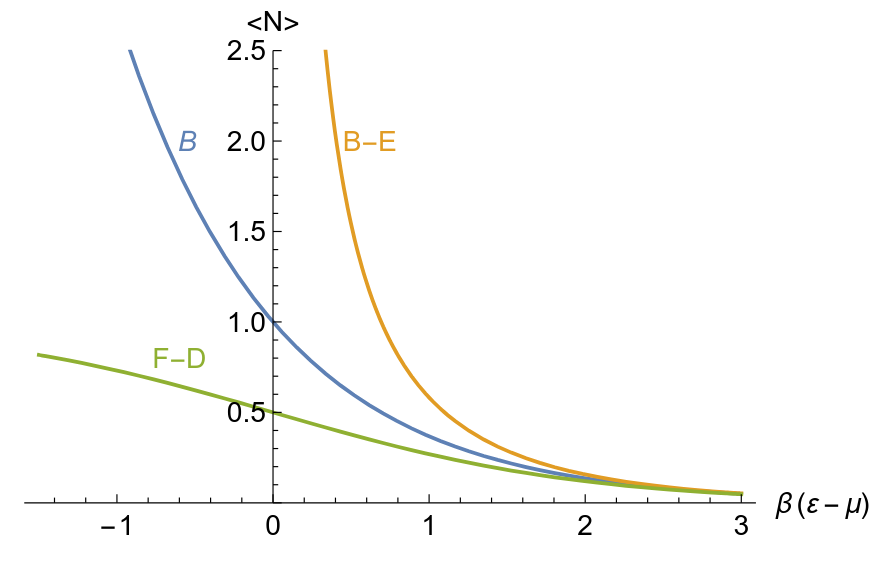
\includegraphics[width=0.45\textwidth]{mo.png}
	\caption{}
	\label{fig:mo}
\end{figure}
In the classical limit, we have that $\mu << 1$, $\varepsilon_r > \varepsilon_r^{\text{min}}$, so $\mu - \varepsilon_r^{\text{min}} << 0$ and $e^{(\mu - \varepsilon)\beta} << 1$. Considering the Taylor expansion of $\ln(1\pm x)$, the grand potential then becomes,
\begin{equation}
	\Phi_G = -k_BTe^{\mu\beta}\sum_r\underbrace{e^{-\varepsilon_r \beta}}_{Z_1}
\end{equation}
we have thus recovered the single particle partition function for a particle in a box, and we'll find $Z_1 = Vg_sn_Q$. We can then find the average particle number,
\begin{equation}
	\langle N \rangle = - \left(\pdv{\Phi_G}{\mu}\right)_{T,V} \approx e^{\mu\beta}Z_1.
\end{equation}
Solving for $\mu$,
\begin{equation}
	\mu = -k_BT\ln\left(\frac{g_sn_Q}{n}\right)
\end{equation}
so for $\mu << 0$, we require $n << n_Q$, as in the classical limit. Knowing that $\Phi_G = F - \mu N$, we have,
\begin{equation}
 	F = -Nk_BT\left(\ln\left(\frac{Z_1}{N}\right)+1\right)
\end{equation}
which is the classical Helmholtz free energy with $Z_N = \frac{(Z_1)^N}{N!}$, allowing us to recover the classical ideal gas. If we inspect the occupancy for $\mu << 0$, we have,
\begin{equation}
	\overline{n}(\varepsilon) \approx N\frac{e^{-\varepsilon\beta}}{Z_1}
\end{equation}
which is the Boltzmann distribution. The Boltzmann, Bose-Einstein, and Fermi-Dirac distributions are plotted as functions of $(\varepsilon - \mu)\beta$ in figure \ref{fig:mo}
\section{Ideal Fermi Gas}
\subsection{Electrons in Metal}
\subsubsection{Zero Temperature Fermi Gas}
\begin{figure}[h]
	\centering
	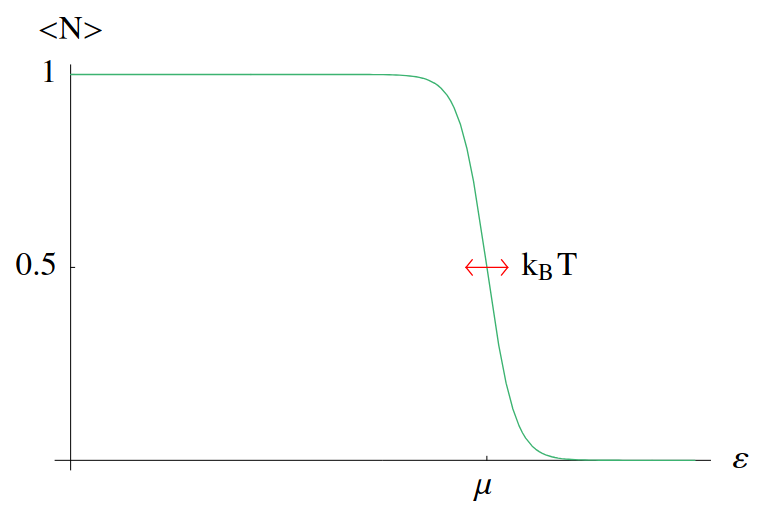
\includegraphics[width=0.5\textwidth]{fermion.png}
	\caption{}
	\label{eq:fermion}
\end{figure}
Electrons are free to move around, but the potential is not constant, and we have wells at each atom position. The free electron model ignores this and treats electrons as moving in a 0 potential box. We then have the same Schrodinger equation solution for each atom, as being an atom in a box. We will also ignore $e^- - e^-$. The electrons in a solid are not classical. The occupancy of electrons will be given by the expression for fermions,
\begin{equation}
	\overline{n}(\varepsilon)  = \frac{1}{e^{(\varepsilon - \mu)\beta}},
\end{equation}
which is plotted in figure \ref{eq:fermion}. All energy levels must be occupied, so we must have $\varepsilon >> k_BT$, so we must consider $\mu << 0$ and the low temperature limit $T \to 0$. In this case, we find that the occupancy approaches a step function,
\begin{equation}
	\overline{n}(\varepsilon) = \Theta(\mu - \varepsilon) = \begin{cases}
		1 & \mu > \varepsilon \\
		0 & \mu < \varepsilon \\
	\end{cases}.
\end{equation}
So, we see that $\mu$ is the highest occupied state at 0 temperature. This is also known as the \textit{Fermi energy}. The corresponding value of $k_f$ is known as the \textit{Fermi momentum}, which (for non-relativistic particles) is related to the Fermi energy by,
\begin{equation}
	\frac{\hbar^2k_f^2}{2m} = \varepsilon_f. \label{eq:fermi_e}
\end{equation}
We can find the value of the Fermi energy by considering,
\begin{equation}
	\begin{split}
		\langle N \rangle = \int_0^{\infty}g(k) \overline{n}(k)\dd{k} &= \int_0^{k_f}g(k)\dd{k} \\
		& = \frac{Vg_s}{2\pi^2}\int_0^{k_f}k^2\dd{k} = \frac{V}{\pi^2}\frac{1}{3}k_f^3.
	\end{split}
\end{equation}
Knowing about equation \eqref{eq:fermi_e} and knowing $n = N/V$, we can write,
\begin{align}
	k_f = (3\pi^2n)^{1/3} && \varepsilon_f = \frac{(3\pi^2\hbar^3n)^{2/3}}{2m}.
\end{align}
The average energy of a fermi gas is given by,
\begin{equation}
	\langle E \rangle  = \frac{V}{\pi^2}\int_0^{k_f}\frac{\hbar^2k^2}{2m}k^2\dd{k} = \frac{3}{5}\langle N \rangle \varepsilon_f.
\end{equation}
All of the above is at zero temperature. We can obtain expressions for pressure and bulk modulus,
\begin{align}
	P=\frac{2}{5}n\varepsilon_f\propto\left(\frac{N}{V}\right)^{\frac{5}{3}} && B = -v\left(\pdv{P}{V}\right)_{T} = \frac{5}{3}P = \frac{2}{3}n\varepsilon_f.
\end{align}
\subsubsection{Finite Temperature Fermi Gas}
As temperature rises, the chemical potential will not remain constant. We will make a change of variables,
\begin{align}
	x = \frac{\hbar^2k^2}{2m}\beta && k=\sqrt{\frac{2m}{\hbar^2}\beta x} && \dd{k} = \frac{1}{2}\sqrt{\frac{2m}{\beta\hbar^2}}x^{-\frac{1}{2}}\dd{x}
\end{align}
and calculate the electron density,
\begin{equation}
	\frac{N}{V} = \frac{1}{2} \left(\frac{2m}{\hbar\beta}\right)^{\frac{3}{2}}\frac{g_s}{2\pi^2}\underbrace{\int_0^{\infty}\frac{x^{\frac{1}{2}}}{\bar{z}e^{x} + 1}} \label{eq:i}
	\end{equation}
where,
\begin{equation}
	\bar{z} = \frac{1}{z}.
\end{equation}
The integrand in equation \eqref{eq:i} is shown as a function of energy at fixed temperature in figure \ref{fig:a}. We can see that as $\bar{z}$ increases, $\mu$ decreases through 0 into negative values. 
\begin{figure}[h]
	\centering
	\begin{subfigure}{0.4\textwidth}
		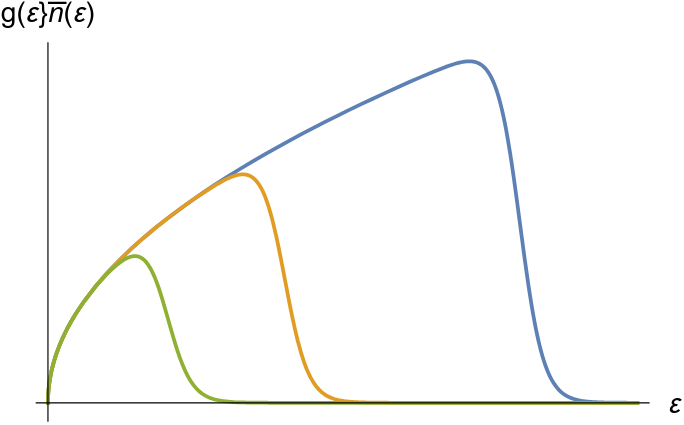
\includegraphics[width=\textwidth]{a1.png}
		\label{fig:a1}
		\caption{$\mu > 0$, decreasing from blue to green.}
	\end{subfigure}
	\begin{subfigure}{0.4\textwidth}
		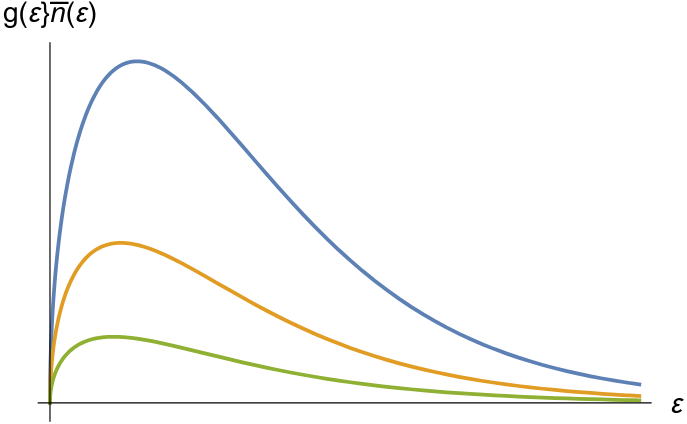
\includegraphics[width=\textwidth]{a2.png}
		\label{fig:a2}
		\caption{$\mu < 0$, decreasing, with blue at $\mu = 0$.}
	\end{subfigure}
	\caption{}
	\label{fig:a}
\end{figure}
\noindent
We can rearrange \eqref{eq:i} to get,
\begin{equation}
	F(\bar{z}) = \frac{\sqrt{\pi}}{2}\frac{n}{g_sn_q}
\end{equation}
where we note that $\bar{z} \to 0$ is an asymptote. Furthermore, as $\mu << 0$, $F(\hat{z}) \to \frac{\sqrt{\pi}}{2\bar{z}}$ which recovers the classical limit. 
\begin{figure}[h]
\centering
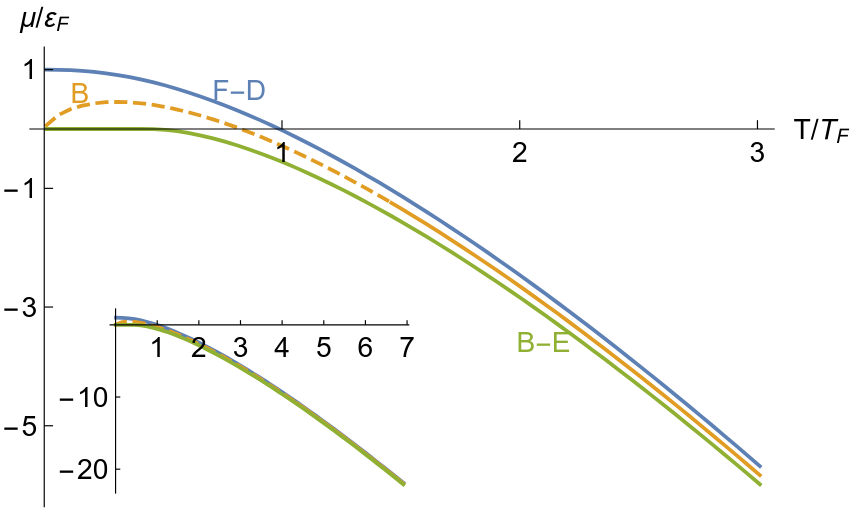
\includegraphics[width=0.425\textwidth]{muef}
\caption{Blue - Fermi Dirac, Orange - Classical Boltzmann, Green - Bose-Einstein}
\label{fig:muef}
\end{figure}
In figure \ref{fig:muef} is plotted the chemical potential as a function of temperature, scaled by the Fermi energy and temperature. We see that the classical approximation approaches the Fermi distribution as $T \to \infty$. If we fix the particle number, we can make an expansion around $T = 0$,
\begin{equation}
	\mu = \varepsilon_f - \frac{\pi^2}{12}\frac{(k_BT)^2}{\varepsilon_f}
\end{equation}
and,
\begin{equation}
	\langle E \rangle = \frac{3}{2}N\varepsilon_f + \frac{N\pi^2}{4}\frac{(k_BT)^2}{\varepsilon_f}
\end{equation}
so we see that both expressions are quadratic in $T$, so temperature dependence is heavily suppressed at the low temperature limit.
\subsubsection{Low Temperature Limit of the Fermi Gas}
Electrons in a metal are all below $T_F$, i.e., $T << T_F$, where $T_F$ is $\sim 80000$K in copper. At 0K, the energy level distribution as seen in figure \ref{fig:a1} would become a ramp, with the step down at $\varepsilon_f$. The reason we see a smooth curve is because electrons which have energies $\sim\varepsilon_f$ are overcome by thermal effects and are brought to energy levels above $\varepsilon_f$. The width of energies at which this happens is $\sim nk_BT\times g(\varepsilon_f)$, where n is a number of the order of a few. The electrons near 0K will have an energy equal to that at $0$K, plus an additional energy due to thermal effects,
\begin{equation}
	E(T) = E(0) + n(k_BT)^2g(\varepsilon_f).
\end{equation}
We have that,
\begin{align}
	\varepsilon_f = \frac{\hbar^2}{2m}\left(3\pi^2\frac{N}{V}\right)^{2/3} && g(\varepsilon_f) = \frac{3}{2}N\varepsilon_f^{-1}
\end{align}
so,
\begin{equation}
	E(T) = E(0) + \sim \underbrace{N\frac{(k_BT)^2}{\varepsilon_F}}_{Nk_BT\left(\frac{T}{T_F}\right)}
\end{equation}
so we see that the fractional variation is also heavily suppressed, and that the additional energy is $\propto T^2$. 
\subsubsection{Thermal Properties}
If we consider the the heat capacity at constant volume, $C_V^{\text{electronic}} \sim Nk_B\left(\frac{N}{k_B}\right)$ which is linear in $T << Kk_B$. Furthermore, at low temperature is $C_V^{\text{lattice}} \sim T^3$, so we  see that the electronic contribution is heavily suppressed, as expected. We can model the heat capacity as,
\begin{equation}
	\frac{C_V}{T} = a + bT^2.
\end{equation}
We can relate thermal conductivity to electrical conductivity by the Wiedemann-Franz law,
\begin{equation}
	\frac{\kappa}{\sigma} = LT
\end{equation}
where the thermal conductivity and electrical conductivity for a gas are given by,
\begin{align}
	\kappa = \frac{1}{3}\langle v\rangle^2\tau C_V^{\text{el}} && \sigma = \frac{ne^2\tau}{m_e}
\end{align}
where $\tau$ is the relaxation time, given by $\tau = \lambda/\langle v \rangle$ where $\lambda$ is the mean free path. We can then write the Wiedemann-Franz law as,
\begin{equation}
	\frac{\kappa}{\sigma} \frac{k_B\pi^2}{3e^2}T.
\end{equation}
\subsubsection{Magnetic Properties}
In contrast to expectation, at any temperature we find the average magnetic moment is independent of $T$ and much smaller than expected if each electron were free to orient in the field. Applying a magnetic field causes the electrons to occupy more states in spin up or spin down, resulting in a magnetic moment of,
\begin{equation}
	m = \frac{3}{2}N\mu_B \frac{N_BB}{\varepsilon_f}.
\end{equation}
\subsection{White Dwarf Stars}
As fuel runs out, stars cool and contract. This leads to gravity being countered by the pressure of a dense fermi gas which is approximately degenerate ($0$K). Although still hot, the density is such that $\mu >> k_BT$. If we assume non-relativistic particles, we can say $M_* = M_{\odot}/2$. We then have,
\begin{align}
	N = \frac{2M_*}{M_{\text{He}}} && V = \frac{4\pi}{3}R_*^3
\end{align}
so,
\begin{equation}
	n \propto \frac{M_*}{M_{\text{He}}}
\end{equation}
and,
\begin{equation}
	E = \frac{3}{2}\varepsilon_f \propto n^{2/3}
\end{equation}
thus,
\begin{equation}
	E \propto M_{*}\left(\frac{M_*}{R_*^3}\right)^{2/3} = a \frac{M_*^{5/3}}{R_*}
\end{equation}
and the gravitational energy is,
\begin{equation}
	E_G = -\underbrace{\frac{3}{5}G}_{b} \frac{m_*^2}{R_*}.
\end{equation}
This reaches equilibrium when $P$ is at a minimum, or when,
\begin{equation}
	\dv{E}{R_*} = 0 = -2a\frac{M_*^{5/3}}{R_*^3} + b\frac{M_*^2}{R_*^2} \implies R_*M_*^{1/3} = \text{Const}
\end{equation}
which is the mass-radius relation for a white dwarf.
\\\\
As $M_* \to M_{\odot}$, electrons start to become relativistic. In the limit of highly relativistic electrons, $\varepsilon_f \propto k_f \propto n^{1/3}$. The electronic energy is then,
\begin{equation}
	E_{\text{el}} \propto M_*\left(\frac{M_*}{R_*^3}\right)^{1/2} = a'\frac{M_*^{4/3}}{R_*}
\end{equation}
thus, equilibrium collapse is not connected by degeneracy pressure. At the point where the gravitational energy is approximately equal to the electronic energy, we find an upper limit to the mass of a white dwarf,
\begin{equation}
	E_{G} \sim E_{\text{el}} \implies M_* \sim \left(\frac{\hbar c}{G}\right)^{3/2}\frac{1}{(2m_p)^2} = 1.4M_{\odot}
\end{equation}
which is known as the Chandra-Sakar limit. What this means is that no star heavier than the Chandra-Sakar limit can be supported by Fermi pressure. For $M_* \lesssim 2M_{\odot}$, further collapse is halted by neutron degeneracy pressure, and neutron stars are formed.
\section{Ideal Bose Gas}
\subsection{Classical Cavity Radiation}
For a cuboidal cavity of sides $L_x$, $L_y$, and $L_z$, the wave vector for radiation is given by,
\begin{equation}
	\vb{k} = \left(\frac{n_x\pi}{k_x} + \frac{n_y\pi}{k_y} + \frac{n_z\pi}{k_z}\right) \hspace{1em} n_x,n_y,n_z \in \mathbb{Z}.
\end{equation}
$\vb{k}$ determines the modes, which will then have a further 2 distinct modes of polarisation per mode. We would classically expect $k_BT$ per mode for the energy, as there are 2 quadratic degrees of freedom. However, when we apply this, noting we get $g(\omega)$ from $g(k)$ by $\omega = ck$,
\begin{align}
	u(\omega)\dd{\omega} & = k_BT \frac{g(\omega)}{V}\dd{\omega}\\
	u(\omega) & = \frac{k_BT}{\pi^2c^3}\omega
\end{align}
however, this is \textbf{incorrect}. There is no upper limit to $\omega$, so we get infinite energy integrating over all energy. This is known as the "UV catastrophe".
\subsection{Photons and Blackbody Radiation}
\begin{figure}[h]
	\centering
	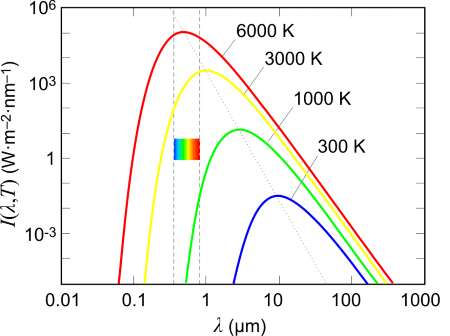
\includegraphics[width=0.4\textwidth]{planck.png}
	\caption{}
	\label{fig:plank}
\end{figure}
Max Planck corrected this model by supposing quantised energy $E = \hbar \omega$. If we consider a single mode,
\begin{equation}
	\langle E \rangle = \frac{\hbar\omega}{e^{\hbar\omega\beta} - 1}
\end{equation}
which we notice is the Bose-Einstein distribution with $\mu = 0$. From this, we can extract \textit{Planck's radiation law},
\begin{equation}
	u(\omega) = \frac{g(\omega)}{V}\frac{\hbar\omega}{e^{\hbar \omega \beta} - 1} = \frac{\hbar}{\pi^2 c^3}\frac{\omega^2}{e^{\hbar\omega\beta} -1}
\end{equation}
which is plotted in figure \ref{fig:plank}. These quanta of energy are photons, which act as bosons with $\mu = 0$. We require,
\begin{align}
	\bar{n}(\omega) = \frac{1}{e^{\hbar\omega\beta}-1} && u(\omega) = \frac{g(\omega)}{V}\hbar\omega\bar{n}(\omega).
\end{align}
A blackbody is obtained by the emission from a small hole in the cavity. Photons all travel at $c$, so radiation has the same spectrum as the cavity radiation. The flux of emitted radiation is given by,
\begin{equation}
	F(\omega) = \frac{c}{4}u(\omega)
\end{equation}
and the total luminosity,
\begin{equation}
	\begin{split}
	L &= \frac{A}{4\pi^2c^2}\int_0^{\infty}\frac{\hbar\omega^3}{e^{\hbar\omega\beta}-1}\dd{\omega}\\
	&= \frac{A(k_BT)^4}{4\pi^2\hbar^3c^2}\underbrace{\int_0^{\infty}\frac{x^3}{e^{\hbar x} -1}\dd{x}}_{\frac{\pi^4}{15}}
	\end{split}
\end{equation}
but recalling Stefan's law, $L = \sigma A T^4$, we can recover a predicted value for the Stefan-Boltzmann constant,
\begin{equation}
	\sigma = \frac{\pi^2k_B^4}{60\hbar^3c^2}.
\end{equation}
Let us recall for ultrarelativistic particles in 3D, $\Phi_G= \frac{1}{3}\langle E \rangle$. we can then write,
\begin{align}
	\langle E \rangle = V\int u(\omega)\dd{\omega} = \frac{4\sigma}{c}VT^4 && P = \frac{4\sigma}{c}T^4 && S = -\dv{\Phi_G}{T} = \frac{16\sigma}{3c}VT^4.
\end{align}
\subsection{Bosons and The Bose-Einstein Condensate}
\end{document}
